\documentclass[tikz,border=2pt]{standalone}

\usepackage{pgfplots}
\usepackage{amsmath}
\pgfplotsset{compat=1.18}

\definecolor{mainBlue}{RGB}{35,90,150}
\definecolor{lightBlue}{RGB}{226,236,247}
\definecolor{softGray}{RGB}{120,120,120}

\begin{document}

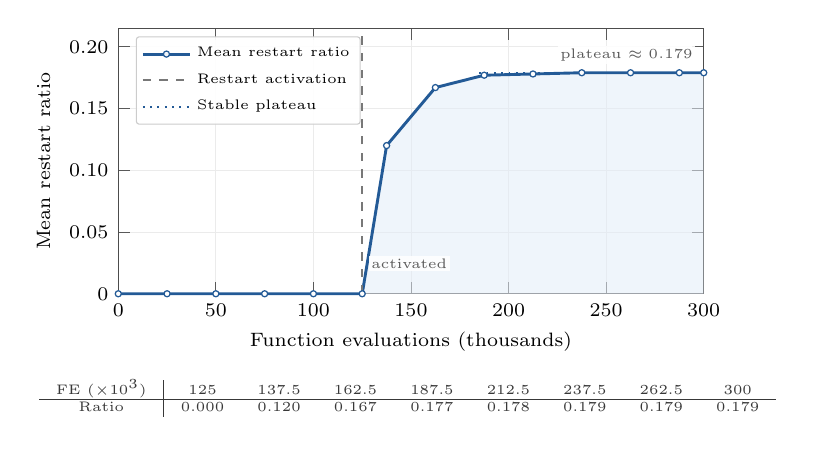
\begin{tikzpicture}

    \begin{axis}[
            name=mainplot,
            width=3.55in,
            height=1.95in,
            xmin=0,
            xmax=300,
            ymin=0,
            ymax=0.215,
            xlabel={Function evaluations (thousands)},
            ylabel={Mean restart ratio},
            xlabel style={font=\scriptsize, yshift=1pt},
            ylabel style={font=\scriptsize},
            tick label style={font=\scriptsize},
            xtick={0,50,100,150,200,250,300},
            ytick={0,0.05,0.10,0.15,0.20},
            yticklabels={0,0.05,0.10,0.15,0.20},
            scaled ticks=false,
            axis line style={black!70, line width=0.45pt},
            tick style={black!65, line width=0.35pt},
            major grid style={black!8, line width=0.32pt},
            grid=major,
            enlarge x limits=false,
            clip=false,
            legend style={
                    at={(0.03,0.97)},
                    anchor=north west,
                    font=\tiny,
                    draw=black!20,
                    fill=white,
                    fill opacity=0.94,
                    text opacity=1,
                    rounded corners=1pt,
                    inner sep=1.8pt,
                    row sep=0.6pt
                },
            legend cell align=left,
        ]

        % Shaded area under the curve
        \addplot[
            draw=none,
            fill=lightBlue,
            fill opacity=0.55,
            forget plot
        ] coordinates {
                (0,0.000)
                (25,0.000)
                (50,0.000)
                (75,0.000)
                (100,0.000)
                (125,0.000)
                (137.5,0.120)
                (162.5,0.167)
                (187.5,0.177)
                (212.5,0.178)
                (237.5,0.179)
                (262.5,0.179)
                (287.5,0.179)
                (300,0.179)
                (300,0)
                (0,0)
            } \closedcycle;

        % Main curve
        \addplot[
            mainBlue,
            line width=1.05pt,
            mark=*,
            mark size=1.10pt,
            mark options={
                    fill=white,
                    draw=mainBlue,
                    line width=0.45pt
                },
        ] coordinates {
                (0,0.000)
                (25,0.000)
                (50,0.000)
                (75,0.000)
                (100,0.000)
                (125,0.000)
                (137.5,0.120)
                (162.5,0.167)
                (187.5,0.177)
                (212.5,0.178)
                (237.5,0.179)
                (262.5,0.179)
                (287.5,0.179)
                (300,0.179)
            };
        \addlegendentry{Mean restart ratio}

        % Restart activation boundary
        \addplot[
            softGray,
            dashed,
            line width=0.65pt,
        ] coordinates {
                (125,0)
                (125,0.210)
            };
        \addlegendentry{Restart activation}

        % Plateau guide
        \addplot[
            mainBlue,
            dotted,
            line width=0.65pt,
        ] coordinates {
                (185,0.179)
                (300,0.179)
            };
        \addlegendentry{Stable plateau}

        % Minimal annotations only
        \node[
            font=\tiny,
            text=black!65,
            anchor=south west,
            fill=white,
            fill opacity=0.88,
            text opacity=1,
            inner sep=1.0pt
        ] at (axis cs:128,0.018)
        {activated};

        \node[
            font=\tiny,
            text=black!65,
            anchor=south east,
            fill=white,
            fill opacity=0.88,
            text opacity=1,
            inner sep=1.0pt
        ] at (axis cs:296,0.186)
        {plateau $\approx 0.179$};

    \end{axis}

    % ------------------------------------------------------------
    % Compact value strip below the plot
    % ------------------------------------------------------------
    \node[
        anchor=north,
        font=\tiny,
        text=black!78,
        align=center
    ] at ([yshift=-0.38in]mainplot.south) {
        \begin{tabular}{c|cccccccc}
            FE ($\times10^3$) & 125   & 137.5 & 162.5 & 187.5 & 212.5 & 237.5 & 262.5 & 300   \\
            \hline
            Ratio             & 0.000 & 0.120 & 0.167 & 0.177 & 0.178 & 0.179 & 0.179 & 0.179
        \end{tabular}
    };

\end{tikzpicture}

\end{document}